\documentclass[compress,handout]{beamer}
% use handout option for one slide per page
\mode<presentation>

\usetheme{Frankfurt} 
%regular LaTeX title/author info
%\AtBeginSection[]{} % for optional outline or other recurrent slide

\usecolortheme{seahorse}
\definecolor{darkgreen}{rgb}{0,0.7,0}

\usepackage[percent]{overpic}
\newcommand{\eqcolor}{blue} 
\newcommand{\txtcolor}{black} 


\usepackage[T1]{fontenc}
\usepackage[utf8]{inputenc}
\usepackage{lmodern}

\usepackage{graphicx}
%\usepackage{float}
\usepackage{amsmath}
% \usepackage{verbatim}
% \usepackage{amssymb} % for fonts like \mathbb
%\usepackage{pstricks}
% \usepackage{tikz}	
% \usepackage{hyperref}

% % set up page margins
% \usepackage[left=3cm,right=3cm,top=2cm,bottom=2cm]{geometry}

% circuits diagrams
% \usepackage[european]{circuitikz}

% linespacing and font
%\usepackage{fontspec}
% \usepackage{setspace}

% this allows include pdf document
% \usepackage{pdfpages}

% allow multirow in tabular environment
\usepackage{multirow}

\usepackage{multicol} 
%: Specific notations 
% Specific notations: highlighted while in draft 
\newcommand{\notcolor}{blue} 

%\newcommand{\+}[2]{\newcommand{#1}[1]{{\color{\notcolor}#2}}} 
\newcommand{\+}[2]{\def#1{{\color{\notcolor}#2}} }
%\newcommand{\1}[2]{\renewcommand{#1}[1]{{\color{\notcolor}#2}}} 
\newcommand{\1}[2]{\def#1##1{{\color{\notcolor}#2}}} 
%\newcommand{\1}[2]{\renewcommand{#1}[1]{#2}} 
%\newcommand{\2}[2]{\newcommand{#1}[2]{{\color{\notcolor}#2}}} 
%\newcommand{\3}[2]{\newcommand{#1}[3]{{\color{\notcolor}#2}}}

\newcommand{\Fig}[1]{Figure~\ref{fig:#1}}
\newcommand{\fig}[1]{Fig.~\ref{fig:#1}}
\newcommand{\Tab}[1]{Table~\ref{tab:#1}}
\newcommand{\tab}[1]{Tab.~\ref{tab:#1}}


% define arrows for Markov chain diagrams
% general right to left double harpoon
% define four connection position #5 and connect the arrows in +-5degrees
% first parameter define origin node 
% second parameter define destination node,
% third parameter label of top arrow
% fourth parameter label of bottom arrow
% fifth parameter define connection point - angle in degrees on the origin node
\newcommand{\leftrightdoubleharpoon}[5]{
    \draw[-left to,thick] ({#1}.{#5+5}) -- node[above] {\scriptsize #3} ({#2}.{#5+175});
    \draw[left to-,thick] ({#1}.{#5+355}) -- node[below] {\scriptsize #4} ({#2}.{#5+185});
}
% general up to down harpoon
 \newcommand{\updowndoubleharpoon}[5]{
     \draw[-left to,thick] ({#1}.{#5+5}) -- node[left] {\scriptsize #3$\hspace{0.3em}$} ({#2}.{#5+175});
     \draw[left to-,thick] ({#1}.{#5+355}) -- node[right] {\scriptsize $\hspace{0.2em}$#4} ({#2}.{#5+185});
}

% general up to down harpoon -- DASHED VARIANT
 \newcommand{\updowndoubledashedharpoon}[5]{
     \draw[-left to,dashed] ({#1}.{#5+5}) -- node[left] {\scriptsize #3$\hspace{0.3em}$} ({#2}.{#5+175});
     \draw[left to-,dashed] ({#1}.{#5+355}) -- node[right] {\scriptsize $\hspace{0.2em}$#4} ({#2}.{#5+185});
}

% general down to up harpoon
 \newcommand{\downupdoubleharpoon}[5]{
     \draw[-right to,thick] ({#1}.{#5-5}) -- node[left] {\scriptsize $\hspace{0.2em}$#3} ({#2}.{#5-175});
     \draw[right to-,thick] ({#1}.{#5-355}) -- node[right] {\scriptsize #4$\hspace{0.3em}$} ({#2}.{#5-185});
}

% style for the differential equations
\renewcommand{\d}{{\mathrm{d}}}

\newcommand{\df}[2]{\frac{\d{#1}}{\d{#2}}}
\newcommand{\ddf}[2]{\frac{\d^2 {#1}}{\d{#2}^2}}
\newcommand{\ddt}[1]{\frac{\d {#1}}{\d{\t}}}

\newcommand{\mat}{\boldsymbol}
\newcommand{\T}{^{\color{\notcolor}\!\top}} % matrix transposition 
\providecommand{\norm}[1]{\lVert#1\rVert}

% cell model variables
\+{\vm}{V} % membrane voltage
\+{\ina}{\mathrm{I_{Na}}}
\+{\ical}{\mathrm{I_{Ca(L)}}}
\+{\irel}{\mathrm{I_{rel}}}
\+{\caiss}{\mathrm{[Ca^{2+}]_{ss}}}
\+{\cajsr}{\mathrm{[Ca^{2+}]_{JSR}}}
\+{\cai}{\mathrm{[Ca^{2+}]_i}}
\+{\nai}{\mathrm{[Na^+]_i}}
\+{\ki}{\mathrm{[K^+]_i}}
\+{\csqn}{[\mathrm{CSQN}]}
\+{\csqnbar}{\mathrm{\overline{CSQN}}}

% chemical elements
\+{\Ca}{\mathrm{Ca}}
\+{\Caion}{$\mathrm{Ca^{2+}}~$}

% physical units
\+{\mus}{\mathrm{\mu s}} % micro seconds
\+{\mV}{\mathrm{mV}} % milivolts
\+{\mMol}{\mathrm{mM}} % miliMol/L
\+{\muM}{\mathrm{\mu M}} % microMol/L
\+{\ms}{\mathrm{ms}} % miliSecond
\+{\muA}{\mathrm{\mu A}} % microAmper
\+{\muF}{\mathrm{\mu F}} % microFarad

% methods' options
\+{\stT}{\Delta t} % time step

% functions
\+{\abs}{\mathrm{abs}} % absolute value

% shortcuts for transition rates
\1{\alp}{\alpha_{#1}}
\1{\bet}{\beta_{#1}}
\1{\gam}{\gamma_{#1}}
\1{\del}{\delta_{#1}}

\1{\lam}{\lambda_{#1}}
\1{\phis}{\phi_{#1}}
\1{\ome}{\omega_{#1}}

\+{\ConeCtwo}{\alp{1R}}
\+{\CtwoCthree}{\alp{2R}}
\+{\CthreeCfour}{\alp{3R}}
\+{\CfourOone}{\alp{4R}}

\+{\IoneItwo}{\alp{1R}}
\+{\ItwoIthree}{\alp{2R}}
\+{\IthreeIfour}{\alp{3R}}
\+{\IfourIfive}{\alp{4R}}
          
\+{\CtwoCone}{\bet{1R}}
\+{\CthreeCtwo}{\bet{2R}}
\+{\CfourCthree}{\bet{3R}}
\+{\OoneCfour}{\bet{4R}}

\+{\ItwoIone}{\bet{1R}}
\+{\IthreeItwo}{\bet{2R}}
\+{\IfourIthree}{\bet{3R}}
\+{\IfiveIfour}{\bet{4R}}

\+{\ConeIone}{\gam{1R}}
\+{\CtwoItwo}{\gam{2R}}
\+{\CthreeIthree}{\gam{3R}}
\+{\CfourIfour}{\gam{4R}}
\+{\OoneIfive}{\gam{5R}}
          
\+{\IoneCone}{\del{1R}}
\+{\ItwoCtwo}{\del{2R}}
\+{\IthreeCthree}{\del{3R}}
\+{\IfourCfour}{\del{4R}}
\+{\IfiveOone}{\del{5R}}

\+{\Cone}  {C_{1}}
\+{\Ctwo}  {C_{2}}
\+{\Cthree}{C_{3}}
\+{\Cfour} {C_{4}}
\+{\Oone}  {O}
\+{\Ione}  {I_{1}}
\+{\Itwo}  {I_{2}}
\+{\Ithree}{I_{3}}
\+{\Ifour} {I_{4}}
\+{\Ifive} {I_{5}}


\+{\mA}{\mat A}
\+{\mB}{\mat B}
\+{\mC}{\mat C}
\+{\mM}{\mat M}
\+{\c}{c}
\+{\u}{u}
\+{\vv}{v} % \v is reserved for hacek
\+{\w}{w}
\+{\x}{x}
\+{\y}{y}
\+{\ybar}{\bar{y}}
\+{\dt}{\Delta t}
\+{\dt}{\stT}
\+{\tC}{\tau}
\+{\t}{t}


% \+{\dt}{h}

% for MC diagrams                               
\usepackage{tikz}                               
\usetikzlibrary{arrows}                         

\usepackage{dcolumn} % for decimal point column alignment in tables

%: Specific notations 
% Specific notations: highlighted while in draft 
% \newcommand{\CAH}[1]{{\boldsymbol{\color{magenta}#1}}}
% \newcommand{\CAL}[1]{{\boldsymbol{\color{cyan}#1}}}
% \newcommand{\CAS}[1]{{\boldsymbol{\color{darkgreen}#1}}}

\everymath{\color{\eqcolor}}


%%%%%%%%%%%%%%%%%%%%%%%%%%%%%%%%%%%%%%%%
% http://tex.stackexchange.com/questions/33969/changing-font-size-of-selected-slides-in-beamer
% \usepackage{lipsum} % lorem ipsum

% \newcommand\Fontvi{\footnotesize\selectfont}
%%%%%%%%%%%%%%%%%%%%%%%%%%%%%%%%%%%%%%%%


\title{Analysis of Numerical Methods for Markov Chain Models of Ionic Channels}
\author{Tom\'a\v s Star\'y, Vadim N. Biktashev }
\institute{\footnotesize 
  College of Engineering, Mathematics and Physical Sciences \\[1ex]
  \includegraphics[width=0.3\linewidth]{fig/exeLogo.pdf} 
}
\date{\it
  British Applied Mathematics Colloquium, Oxford, \\
  Fri 8 Apr, 2016
}


% \useoutertheme[subsection=false]{smoothbars}

% \setbeamertemplate{note page}[plain]

% \newcommand{\compresslist}{ % Define a command to reduce spacing within itemize/enumerate environments, this is used right after \begin{itemize} or \begin{enumerate}
% \setlength{\itemsep}{1pt}
% \setlength{\parskip}{0pt}
% \setlength{\parsep}{0pt}
% }

\newcommand{\highlight}[1]{\boxed{#1}}

\begin{document}
 
% title page
\frame{	\titlepage }

% outline
% \section[Outline]{}
% \frame{\tableofcontents}

% \subsection{Cellular Membrane}

\section{Introduction}
\subsection{Cellular Membrane}
\begin{frame}
  \frametitle{Cellular Membrane}
  Capacitor equation describing a single cell
  {\color{\eqcolor}
  \begin{align*}
    \ddt{\vm} = -\frac{1}{\Cm} \sum_{k} \Im_k(\vm,\c,\Pop)
  \end{align*}}
      \vspace{-1.5em}
  \begin{itemize}
  \item $\vm(t)$, $\Cm$  -- membrane voltage and capacitance
  \item $\Im_k(\vm,\c,\Pop)$ -- ionic currents
  \item $\c(t)$ -- ionic concentrations
  \item $\Pop(t)$ -- open probability of ionic channel
  \end{itemize}
\end{frame}



%%%%%%%%%%%%%%%%%%%%%%%%%%%%%%%%%%%%%%%%%%%%%%%%%%
\subsection{Ion Channel}
\begin{frame}
  \frametitle{Ion Channel}
  % Composed of {\em gates}:
  % {\color{\eqcolor}
  %   \begin{align*}
  %     \ddt{\y} = \alpha(\vm) (1-\y) - \beta(\vm) \y 
  %   \end{align*}}
  % % 
  % \begin{itemize}
  % \item $\y$ -- open probability of the gate

  % \item $\alpha$ -- opening transition rate
  % \item $\beta$ -- closing transition rate
  % \item $\vm$ -- membrane voltage
  % \end{itemize}
  % %
  % \uncover<2>{
  % Generalized by
  {\em Markov chain} states
  {\color{\eqcolor}
    \begin{align*}
      \ddt{\vec \x} = \mM(\vm,\c)\, \vec \x
    \end{align*}}
        \vspace{-1.5em}
  % 
  \begin{itemize}
  \item $\vec\x$ -- conductive (open) and non-conductive states:
    {\color{\eqcolor}$$\Pop(t) = \sum\x_\mathrm{open}$$}
      \vspace{-1.5em}
  \item $\mM$ -- transition rates matrix
  \end{itemize}
  % }% uncover 2

  \uncover<2->{
  Time-stepping through time discretization $\t_n = \t_0 + n \dt$ \\
  e.g. simplest -- forward Euler method:
  {\color{\eqcolor}
    \begin{align*}
      \vec\x_{n+1} = \vec\x_n + \dt \ddt{\vec\x_n}
    \end{align*}}
  %
  \vspace{-1.5em}
  \begin{multicols}{2}
    \begin{itemize}
    \item $\vec\x_n\approx\vec\x(\t_n)$
    \item $\dt$ -- time step
    \end{itemize}
  \end{multicols}
  }
  \uncover<3->{\emph{Numerically unstable} for large $\dt$.\\[1.5ex]}

\end{frame}

\section{Methods}
\subsection{Exponential Integration}
\begin{frame}
  \frametitle{Exponential Integration}
  % We extend the exponential time differentiation for Markov chain
  Approximation by ``freezing'' $\mM(\vm(t),\c(t))\approx\mM(\vm_n,\c_n)$ gives
  {\color{\eqcolor}
    \begin{align*}
      \vec \x_{n+1} = \exp\left(\mM(\vm_n,\c_n) \dt \right) \vec \x_n 
    \end{align*}}
  \uncover<2->{
    Matrix exponential:
    % 
    {% \scriptsize
      \color{\eqcolor}
      \begin{align*}
        \Tab= \exp\left(\mM \dt \right) =
          \eM\exp{(\eD \dt)}\eM^{-1}
      \end{align*}}
    \begin{itemize}
      \vspace{-0.5em}
    \item $\mM = \eM \eD \eM^{-1}$ -- eigenvalue decomposition
    \item matrices: $\eM$ -- e-vectors in columns, $\eD$ -- e-values on diagonal
    \end{itemize}
    }% uncover 2
    \uncover<3->{
      Tabulation:
      \begin{itemize}
      \item save $\eM(\vm_j), \eD(\vm_j)$ for a fine grid of dependent variable
      \end{itemize}
      }
\end{frame}

\section{Application}
\subsection{Case 1: RyR Channel}

\begin{frame}
  \frametitle{Case 1: RyR Channel}
  \begin{minipage}{0.40\linewidth}
    \begin{tikzpicture}[%node distance=100mm,
state/.style={
% The shape:
circle,minimum size=8mm,rounded corners=2mm,
% The rest
%draw=black
},
scale=1.8
,transform canvas={scale=0.65}
,shift={(0,-1.0)}
]
% draw the nodes
\path
  % bottom row 
(0,0)   node (N00) [state] {$C_1$}
(0.8,0) node (N10) [state] {$C_2$}
(1.6,0) node (N20) [state] {$C_3$}
(2.4,0) node (N30) [state] {$C_4$}
(3.2,0) node (N40) [state] {$O_1$}
  % upper row
(0,0.8)  node (N01) [state] {$I_1$}
(0.8,0.8)  node (N11) [state] {$I_2$}
(1.6,0.8)  node (N21) [state] {$I_3$}
(2.4,0.8)  node (N31) [state] {$I_4$}
(3.2,0.8)  node (N41) [state] {$I_5$};
% draw the transitions
%     \draw[-left to] (N01.280) -- node[left] {$\alpha_i$} (N00.80);
%     \draw[left to-] (N01.260) -- node[right] {$\beta$} (N00.100);
%     arrows up to down

% \uncover<1,2>{
%   \downupdoubleharpoon{N01}{N00}{}{}{-90}
%   \downupdoubleharpoon{N11}{N10}{}{}{-90}
%   \downupdoubleharpoon{N21}{N20}{}{}{-90}
%   \downupdoubleharpoon{N31}{N30}{}{}{-90}
%   \downupdoubleharpoon{N41}{N40}{}{}{-90}
%   % arrows right to left on the bottom row
% \leftrightdoubleharpoon{N00}{N10}{}{}{0}
% \leftrightdoubleharpoon{N10}{N20}{}{}{0}
% \leftrightdoubleharpoon{N20}{N30}{}{}{0}
% \leftrightdoubleharpoon{N30}{N40}{}{}{0}
% % arrows right to left on the top row
% \leftrightdoubleharpoon{N01}{N11}{}{}{0}
% \leftrightdoubleharpoon{N11}{N21}{}{}{0}
% \leftrightdoubleharpoon{N21}{N31}{}{}{0}
% \leftrightdoubleharpoon{N31}{N41}{}{}{0}
% } % uncover 1
% \uncover<3->{
%   \downupdoubleharpoon{N01}{N00}{$\del{1R}$}{$\gam{1R}$}{-90}
%   \downupdoubleharpoon{N11}{N10}{$\del{2R}$}{$\gam{2R}$}{-90}
%   \downupdoubleharpoon{N21}{N20}{$\del{3R}$}{$\gam{3R}$}{-90}
%   \downupdoubleharpoon{N31}{N30}{$\del{4R}$}{$\gam{4R}$}{-90}
%   \downupdoubleharpoon{N41}{N40}{$\del{5R}$}{$\gam{5R}$}{-90}
%   }% uncover 3
%   % arrows right to left on the bottom row
%   \uncover<4>{
% \leftrightdoubleharpoon{N00}{N10}{$\alp{1R}$}{$\bet{1R}$}{0}
% \leftrightdoubleharpoon{N10}{N20}{$\alp{2R}$}{$\bet{2R}$}{0}
% \leftrightdoubleharpoon{N20}{N30}{$\alp{3R}$}{$\bet{3R}$}{0}
% \leftrightdoubleharpoon{N30}{N40}{$\alp{4R}$}{$\bet{4R}$}{0}
% % arrows right to left on the top row
% \leftrightdoubleharpoon{N01}{N11}{$\alp{1R}$}{$\bet{1R}$}{0}
% \leftrightdoubleharpoon{N11}{N21}{$\alp{2R}$}{$\bet{2R}$}{0}
% \leftrightdoubleharpoon{N21}{N31}{$\alp{3R}$}{$\bet{3R}$}{0}
% \leftrightdoubleharpoon{N31}{N41}{$\alp{4R}$}{$\bet{4R}$}{0}
% } % uncover 2

\uncover<-5,7>{\downupdoubleharpoon{N01}{N00}{{\uncover<3,5->{$\del{1R}$}}}{{\uncover<3,5->{$\gam{1R}$}}}{-90}}
\uncover<-5,7>{\downupdoubleharpoon{N11}{N10}{{\uncover<3,5->{$\del{2R}$}}}{{\uncover<3,5->{$\gam{2R}$}}}{-90}}
\uncover<-5,7>{\downupdoubleharpoon{N21}{N20}{{\uncover<3,5->{$\del{3R}$}}}{{\uncover<3,5->{$\gam{3R}$}}}{-90}}
\uncover<-5,7>{\downupdoubleharpoon{N31}{N30}{{\uncover<3,5->{$\del{4R}$}}}{{\uncover<3,5->{$\gam{4R}$}}}{-90}}
\uncover<-5,7>{\downupdoubleharpoon{N41}{N40}{{\uncover<3,5->{$\del{5R}$}}}{{\uncover<3,5->{$\gam{5R}$}}}{-90}}
  % arrows right to left on the bottom row
\uncover<-6>{\leftrightdoubleharpoon{N00}{N10}{{\uncover<3,4,6>{$\alp{1R}$}}}{{\uncover<3,4,6>{$\bet{1R}$}}}{0}}
\uncover<-6>{\leftrightdoubleharpoon{N10}{N20}{{\uncover<3,4,6>{$\alp{2R}$}}}{{\uncover<3,4,6>{$\bet{2R}$}}}{0}}
\uncover<-6>{\leftrightdoubleharpoon{N20}{N30}{{\uncover<3,4,6>{$\alp{3R}$}}}{{\uncover<3,4,6>{$\bet{3R}$}}}{0}}
\uncover<-6>{\leftrightdoubleharpoon{N30}{N40}{{\uncover<3,4,6>{$\alp{4R}$}}}{{\uncover<3,4,6>{$\bet{4R}$}}}{0}}
% arrows right to left on the top row
\uncover<-6>{\leftrightdoubleharpoon{N01}{N11}{{\uncover<3,4,6>{$\alp{1R}$}}}{{\uncover<3,4,6>{$\bet{1R}$}}}{0}}
\uncover<-6>{\leftrightdoubleharpoon{N11}{N21}{{\uncover<3,4,6>{$\alp{2R}$}}}{{\uncover<3,4,6>{$\bet{2R}$}}}{0}}
\uncover<-6>{\leftrightdoubleharpoon{N21}{N31}{{\uncover<3,4,6>{$\alp{3R}$}}}{{\uncover<3,4,6>{$\bet{3R}$}}}{0}}
\uncover<-6>{\leftrightdoubleharpoon{N31}{N41}{{\uncover<3,4,6>{$\alp{4R}$}}}{{\uncover<3,4,6>{$\bet{4R}$}}}{0}};

\end{tikzpicture}    \vspace{3.50em}\\
    \uncover<2->{
    \includegraphics[width=1.0\linewidth]{ryr-tr.pdf}}\\
    \uncover<3->{
      \includegraphics[width=1.0\linewidth]{ryr-inst.pdf}}\\
  \end{minipage}
  \begin{minipage}{0.58\linewidth}
    % \uncover<4->{
    %   \begin{tabular}[t]{l|l|l}
    %   $\caiss(\t)$& $\csqn$& const.\\
    %   \hline
    %   \uncover<5->{$\alp{}$'s}\uncover<8->{, $\gam{}$'s}&
    %   \uncover<7->{$\del{}$'s}&
    %   \uncover<6->{$\bet{}$'s}\\
    % \end{tabular}}
    \uncover<2->{
      Transition rates:
      {\scriptsize
      \color{\eqcolor}
      \begin{align*}
        \mM(\caiss,\csqn)
        \uncover<4->{=
        \left(\begin{array}{l|l}
                \mB & 0 \\\hline 
                0 & \mB 
              \end{array}\right)+}
                    \uncover<5->{\mC}
                    \uncover<4>{\hspace{-1em}\hdots}
      \end{align*}}}
    \uncover<4->{    
      \begin{itemize}
      \item  $\alp{}$'s, $\bet{}$'s -- fast $\mB(\caiss(\t))$
        \uncover<5->{\item $\gam{}$'s, $\del{}$'s -- slow  $\mC(\dots)$}
      % $\norm{\mC(\dots)}\lesssim1\,\ms^{-1}$
    \end{itemize}}
    % Forward Euler limited by instability issues for $dt \ge 7$.
    \uncover<6->{
      Solved in sub-steps as
    {\color{\eqcolor}
    \begin{align*}
      &\vec\vv_{n+1/2}=\exp\left(\dt\,\mB(\t_n)\right)\,\vec\vv_n\\
      &\vec \w_{n+1/2}=\exp\left(\dt\,\mB(\t_n)\right)\,\vec \w_n\\
\uncover<7->{      &\vec\u_{n+1}  =\vec\u_{n+1/2} 
      + \dt\,\mC(\t_n)\,\vec\u_{n+1/2}}
    \end{align*}}
  where $\vec{v}=(I_1, \dots, I_5)$,\\ $\vec{\w}=(C_1,\dots,C_4,O_1)$ 
\uncover<7->{  and $\vec \u =(\vec \vv,\vec \w)$.}}
  \end{minipage}
\end{frame}

\subsection{Case 2: ical Channel}

\begin{frame}
  \frametitle{Case 2: $\ical$ Channel}
  \begin{minipage}{0.50\linewidth}
  \begin{tikzpicture}[%node distance=100mm,
state/.style={
% The shape:
circle,minimum size=8mm,rounded corners=2mm,
% The rest
%draw=black
},
transform canvas={scale=0.53},
scale=2.3,
shift={(0.5,1.2)}]
% draw the nodes
\newcommand{\layer}{}
\newcommand{\calcium}{\mathrm{\layer}}
\newcommand{\open}{O}
{\color{gray}
  \uncover<2,3>{\node[draw,minimum size=6mm] at (-0.8,0) {Mode $\vm$};}
  \uncover<4->{\node[draw,minimum size=6mm] at (-0.8,0) {Single layer};}
\input{layer.tex}}

\uncover<-3>{
\renewcommand{\layer}{Ca}
\renewcommand{\open}{I_{\calcium}}
\begin{scope}[shift={(0,-1.1)}]
  \uncover<2,3>{\node[draw,minimum size=6mm] at (-0.8,0) {Mode $\calcium^{2+}$};}
  \input{layer.tex}
\end{scope}

% draw the transitions betwen Ca and V mode
{\color{lightgray}
  \updowndoubledashedharpoon{00}{Ca00}{{\uncover<3>{$\theta$}}}{{\uncover<3>{$\delta$}}}{-90}
\updowndoubledashedharpoon{10}{Ca10}  {{\uncover<3>{$\theta$}}}{{\uncover<3>{$\delta$}}}{-90}
\updowndoubledashedharpoon{20}{Ca20}  {{\uncover<3>{$\theta$}}}{{\uncover<3>{$\delta$}}}{-90}
\updowndoubledashedharpoon{30}{Ca30}  {{\uncover<3>{$\theta$}}}{{\uncover<3>{$\delta$}}}{-90}
\updowndoubledashedharpoon{40}{Ca40}  {{\uncover<3>{$\theta$}}}{{\uncover<3>{\hspace{-0.25em}$\delta$}}}{-90}
\updowndoubledashedharpoon{51}{Ca51}  {{\uncover<3>{$\theta$}}}{{\uncover<3>{$\delta$}}}{-90}
\updowndoubledashedharpoon{5m1}{Ca5m1}{{\uncover<3>{$\theta$}}}{{\uncover<3>{$\delta$}}}{-90}
}
}

\uncover<5->{
  \begin{scope}[state/.style={
% The shape:
      minimum size=10mm,
% The rest
%draw=black
}]
\node[draw,minimum size=6mm] at (0.8,-1.6) {Mode $\vm$};
\node[draw,minimum size=6mm] at (0.8,-2.4) {Mode $\calcium^{2+}$};
\path 
(1.7,-1.6) node (q1) [state] {$\q$}
(1.7,-2.4) node (q0) [state] {$(1-\q)$};
    \updowndoubledashedharpoon{q1}{q0}{$\theta$}{$\delta$}{-90}
  \end{scope}
}

\end{tikzpicture}

  \end{minipage}
  \begin{minipage}{0.48\linewidth}
    \begin{itemize}
    \item forward Euler instability at $\sim 37$~$\mus$ 
        \uncover<2->{\item two identical layers with \\ $\vm$ dependent transitions}
        \uncover<3->{\item vertical trans. controlled by $\cai$ dependent $\delta$, $\theta$}
          \uncover<4->{
          \item Simplifies as
            \begin{itemize}
            \item a single layer $\ddt{\vec \x} = \mM(\vm) \vec \x $
              % {\color{\eqcolor}
                % \begin{align*}
                %   &\ddt{\vec \x} = \mM(\vm) \vec \x 
                % \end{align*}}
            }
            \uncover<5->{
            \item and a gate model $\ddt{\q} = \theta (1-\q) - \delta \q$
              % \begin{align*}
              %   \hspace{-3em}\ddt{\q} = \theta(\cai) (1-\q) -\\ \delta(\cai) \q
              % \end{align*}
            }
          \end{itemize}

    \end{itemize}
  \end{minipage}\vspace{3.0em}\\
  \uncover<6->{
    \begin{itemize}
    \item Exponential solvers applied for both parts
    \item Open probability $\Pop(t) = \q(t) O(t)$
    \end{itemize}
  }  
\end{frame}

\section{Results and Conclusions}
\subsection{}
\begin{frame}
  \frametitle{Results and Conclusions}
  \includegraphics[width=1.0\linewidth]{summeth.pdf}

    % \begin{minipage}{0.5\linewidth}
      \begin{itemize}
        \uncover<2->{ \item Time step increase from $\sim 6$~$\mus$ to
          $\sim 180$~$\mus$}
        \uncover<2->{\item 27-fold reduction of computational time}
        \uncover<3->{\item time step limited by accuracy requirements}
        \uncover<3->{ \item instability at higher time steps due to non-gating variables ($\nai$ and $\ki$) }
      \uncover<4->{\item addressing instability allows to consider higher order schemes}
      \end{itemize}
  %   \end{minipage}
  % \begin{minipage}{0.48\linewidth}
  %   \uncover<3->{\includegraphics[width=1.0\linewidth]{tab.pdf}}
  % \end{minipage}
\end{frame}

% %%%%%%%%%%%%%%%%%%%%%%%%%%%%%%%%%%%%%%%%%%%%%%%%%%
% \section{Conclusions}

\begin{frame}
\begin{thebibliography}{1}

\bibitem{Hodgkin1952}
A.~L. Hodgkin, A.~F. Huxley.
\newblock A quantitative description of membrane current and its application to
  conduction and excitation in nerve.
\newblock {\em J Physiol} 1952, 117(4):500--544.

\bibitem{Rush1978}
S.~Rush, H.~Larsen.
\newblock A practical algorithm for solving dynamic membrane equations.
\newblock {\em IEEE Trans Biomed Eng} 1978, 25(4):389--392.

\bibitem{Faber2007a}
  Faber GM, Silva J, Livshitz L, Rudy Y.
  \newblock Kinetic properties of the cardiac {L}-type {Ca$^{2+}$} channel and
  its role in myocyte electrophysiology: a theoretical investigation.
  \newblock {\em Biophys J} 2007;\hspace{0pt}92(5):1522--1543.

\bibitem{Stary2015}
  T.~Stary, V.~N.~Biktashev
  \newblock Exponential integrators for a Markov chain model of the fast sodium
  channel of cardiomyocytes.
  \newblock {\em IEEE Trans Biomed Eng} 2015;\hspace{0pt}62(4):1070--1076.

\end{thebibliography}
  
\end{frame}







\begin{frame}
  \frametitle{Cellular Membrane}
  Capacitor equation describing a single cell
  {\color{\eqcolor}
  \begin{align*}
    \ddt{\vm} = -\frac{1}{\Cm} \sum_{k} \Im_k(\vm,\c,\Pop)
  \end{align*}}
  %     \vspace{-1.5em}
  % \begin{itemize}
  % \item $\vm(t)$, $\Cm$  -- membrane voltage and capacitance
  % \item $\Im_k(\vm,\c,\Pop)$ -- ionic currents
  % \item $\c(t)$ -- ionic concentrations
  % \item $\Pop(t)$ -- open probability of ionic channel
  % \end{itemize}
  %     \vspace{1em}
  Ohm's law for current through ionic channel
  {\color{\eqcolor}
  \begin{align*}
    \Im = \Gkmax \Pop(t) \Big[\vm(t) - \Em(c)\Big]
  \end{align*}} 
      \vspace{-1.5em}
  \begin{itemize}
  \item $\Gkmax$ -- maximum conductance 
  \item $\Em(c)$ -- equilibrium voltage for specific ion
  \end{itemize}
\end{frame}

\begin{frame}
  \frametitle{Matrix Exponential}
  % % We extend the exponential time differentiation for Markov chain
  % Approximation by ``freezing'' $\mM(\vm(t),\c(t))\approx\mM(\vm_n,\c_n)$ gives
  % {\color{\eqcolor}
  %   \begin{align*}
  %     \vec \x_{n+1} = \exp\left(\mM(\vm_n,\c_n) \dt \right) \vec \x_n 
  %   \end{align*}}
    Matrix exponential:
    % 
    {% \scriptsize
      \color{\eqcolor}
      \begin{align*}
        &\Tab= \exp\left(\mM \dt \right) =
          \sum_{\Ej = 0}^{\infty} \frac{\mM^\Ej \dt^\Ej}{\Ej!}
          \uncover<2->{ = \sum_{\Ej = 0}^{\infty} \frac{(\eM \eD \eM^{-1})^\Ej \dt^\Ej}{\Ej!}}
          \uncover<3->{
          =\\ &\sum_{\Ej = 0}^{\infty} \frac{ \eM \eD \eM^{-1} \eM \eD \eM^{-1} \hdots \eM \eD \eM^{-1}\dt^\Ej}{\Ej!}
                =\sum_{\Ej = 0}^{\infty} \frac{ \eM  \eD \eD \hdots \eD  \eM^{-1}\dt^\Ej}{\Ej!}
                =\\ &\eM\left(\sum_{\Ej = 0}^{\infty} \frac{ \eD^\Ej  \dt^\Ej}{\Ej!}\right)\eM^{-1}}
                                                \uncover<4->{=
                                                \highlight{\eM\exp{(\eD \dt)}\eM^{-1}}
                                                }
      \end{align*}}
    \begin{itemize}
      \vspace{-0.5em}
      \uncover<2->{\item $\mM = \eM \eD \eM^{-1}$ -- eigenvalue decomposition
      \item matrices: $\eM$ -- e-vectors in columns, $\eD$ -- e-values on diagonal}
      \uncover<3->{\item $\eM^{-1} \eM = \I$ -- identity matrix}
      \uncover<3->{\item $\I\eD = \eD$}
  \end{itemize}
\end{frame}

\subsection{Tabulation}
\begin{frame}
  \frametitle{Tabulation}
  To avoid expensive e-values and e-vectors computations at each time step:
    \begin{itemize}
    \uncover<2->{\item save the matrices $\eM(\tvm_j)$ and $\eD(\tvm_j)$ for a fine grid
      of dependent variable% : $\tvm = (-100, 70)$~mV
      % with the step $\dvm = 0.01$~mV ($\tvm_j=\tvm_\mathrm{min} +j\dvm$)
    }
    \uncover<3->{\item find matrix exponential before the integration \\ $\Tab(\tvm) =
      \eM(\tvm) \exp\left( \eD(\tvm) \dt\right)
      \eM^{-1}(\tvm)$}
    \uncover<4->{\item numerical scheme:
      {\color{\eqcolor}
      \begin{align*}
        \color{\eqcolor}
        \vec \x_{n+1} = \Tab(\tvm_{j(n)}) \vec \x_n
      \end{align*}}
    where $\tvm_{j(n)} \approx \vm_n$.}
    \end{itemize}
\end{frame}




\end{document}
